\newpage
\subsection{Sistema di controllo proporzionale}

\begin{wrapfigure}[11]{r}{0.5\textwidth}
\centering
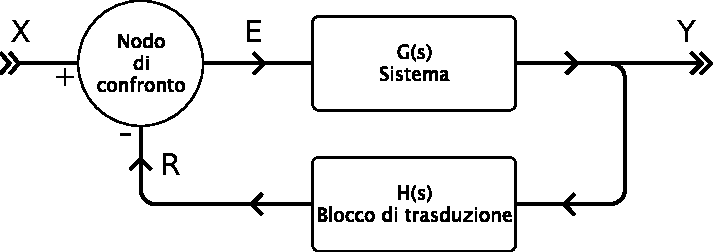
\includegraphics[width=.5\textwidth]{../E06/latex/s2.pdf}
\caption{Schema logico del sistema di controllo proporzionale di temperatura.}
\label{fig5:scheme2}
\end{wrapfigure}

Aggiungiamo ora al circuito proposto nel paragrafo precedente un sistema di controllo proporzionale, la cui funzione sarà quella di riscaldare una resistenza fino a raggiungere una data temperatura di soglia.

Per comprenderne meglio l'implementazione, generalizziamo prima il concetto di controllo proporzionale.
Osserviamo lo schema in Figura \ref : dati due segnali in ingresso X e R , il sistema deve rispondere con Y  se viene rispettata una condizione controllata dal nodo di confronto.
Quest'ultimo avrà dunque il compito di confrontare X ed R e verificare che la condizione, in generale funzione dei due segnali, sia rispettata.
L'aggiornamento di tale condizione è invece affidato al blocco di retroazione, che varia R.

Nel nostro caso, X è la tensione relativa alla temperatura di soglia ($T_{S}$) e R la tensione relativa alla temperatura misurata dalla termoresistenza ($T$).
La nostra Y sarà una data potenza dissipata su una resistenza di potenza che, se posta vicino alla PT100, varierà R, cioè la temperatura letta.
Dobbiamo ora identificare i blocchi relativi al sistema di controllo proporzionale e progettare quelli mancanti nel circuito attuale.

Affidiamo il compito di blocco di retroazione al circuito finora costruito: questo restituisce un valore di tensione proporzionale alla temperatura letta dalla termoresistenza, che dovrà essere confrontato con la soglia.
Successivamente, il blocco di controllo deve fare la differenza fra questi due valori e, una volta raggiungo un valore impostabile, diminuire il valore della corrente fornita alla resistenza di potenza in maniera proporzionale ad E.
Definiamo dunque E=X-R, e per effettuare tale operazione utilizziamo un amplificatore differenziale .
Infine, per fornire la corrente necessaria alla resistenza, utilizzeremo un transistor.

\subsubsection{Blocco di confronto}

Analizziamo il blocco di retroazione in Figura \ref .
Con il trimmer impostiamo una tensione $V_{S}$ proporzionale a $T_{S}$ (bisogna rispettare l'output del circuito precedente per impostarla, cioè $100$\si{\milli\volt\per\celsius}) che può essere confrontata direttamente con la tensione $V_{T}$ relativa a $T$ in arrivo dal blocco di retroazione.
Inoltre, ponendo le resistenze uguali a $1$ \si{\kilo\ohm} e $100$ \si{\kilo\ohm} nel circuito di retroazione dell'amplificatore come in Figura, otteniamo un guadagno $G=100$.

Definiamo la tensione in uscita dall'operazionale come $V_{err}$ e
$$\Delta T = \frac{|V_{T}-V_{S}|}{100\si{\milli\volt\per\celsius}}= | T - T_{S} | $$
Ovviamente, per valori di tensione in entrata maggiori di $\approx 0.15$\si{\volt}, l'opamp entrerà in saturazione, mandando $V_{err}\approx 15$\si{\volt}; altrimenti l'amplificazione sarà quella di un amplificatore invertente.
Dunque varrà la seguente equazione

\begin{equation}
V_{err} = \bigg \{
\begin{array}{rl}
G V_{T} & \mathrm{se} \quad 0<V_{T}<0.15 \si{\volt} \\
\approx 15 \si{\volt} & \mathrm{se} \quad V_{T}>0.15 \si{\volt} \\
\end{array}
\label{eq6:exit_opamp}
\end{equation}

\subsubsection{Sistema}

Per progettare il sistema di riscaldamento proporzionale, dobbiamo fornire potenza (ad una resistenza capace di sopportare alti valori della stessa, detta \textit{resistenza di potenza}) in maniera proporzionale ad E, cioè $\Delta T$.
Per fare ciò, utilizzeremo un transistor 2N2222A con emettitore collegato a comune, le cui caratteristiche sono le seguenti
$$\begin{array}{rl}
\beta = \frac{I_c}{I_b} = 75\\
V_{CE}^{sat}=0.4 \si{\volt}\\
V_{BE}=1.3 \si{\volt}\\
\end{array}
$$
Vale che, con una resistenza di potenza $R_{P} = 27$ \si{\ohm} e impostata una tensione di $5$ \si{\volt} costante ad uno dei suoi capi\footnote{Il REF02 non avrebbe potuto erogare la corrente necessaria a mantenere invariata la tensione ai capi della resistenza.
Dunque, per gestire questa tensione, abbiamo utilizzato il generatore di tensione costante Agilent.
Inoltre, per questo motivo, la comune utilizzata per questo blocco è stata posta indipendentemente per poi essere collegata a quella degli altri blocchi.} come in Figura \ref ,
$$I_{C}=\frac{5 \si{\volt}- V_{CE}^{sat}}{R_P}=170 \si{\milli\ampere}$$
quindi $I_B=I_{C}/\beta=2.27$\si{\milli\ampere}, da cui otteniamo il valore per cui il transistor si trova in saturazione (cioè quando la tensione base emettitore è maggiore di $V_{BE}$ e la tensione base collettore è minore di $V_{CE}^{sat}$)
$$R_B=\frac{V_{err} - V_{BE}}{I_B}=2.2 \si{\kilo\ohm}$$

Considerando il seguente sistema che descrive il transistor nelle condizioni di saturazione e le resistenze calcolate in precedenza
$$
V_{err} = \begin{cases}
\begin{array}{rl}
5\si{\volt}-V_{CE}^{sat} \leq I_{C}R_P\\
I_C=\beta I_B \\
V_B - V_E \geq V_{BE}\\
V_{err}-V_B=I_B R_B
\end{array}
\end{cases}
$$
si può ottenere la condizione di saturazione come una condizione su $V_{err}$
$$V_{err}\geq \frac{5\si{\volt}-V_{CE}^{sat}}{\beta} \frac{R_B}{R_P}+V_{BE} \cong 6.3 \si{\volt}$$
Per tensioni minori il transistor si porterà in regione lineare e, per valori di $V_{err}$ molto bassi, in interdizione.
Dunque, il massimo della corrente (per la legge di Joule il massimo della potenza dissipata), data (\ref{eq6:exit_opamp}), si avrà sicuramente per $\Delta T > 1.5 \si{\celsius}$.
Possiamo dunque affermare di aver impostato il nostro circuito per disabilitare la dissipazione di potenza entro $\approx 0.63$ \si{\celsius} da $T_{S}$.

COMMENTARE il commento per caso a casa di casa con casa a caso

\begin{figure}[ht]
 \centering
   {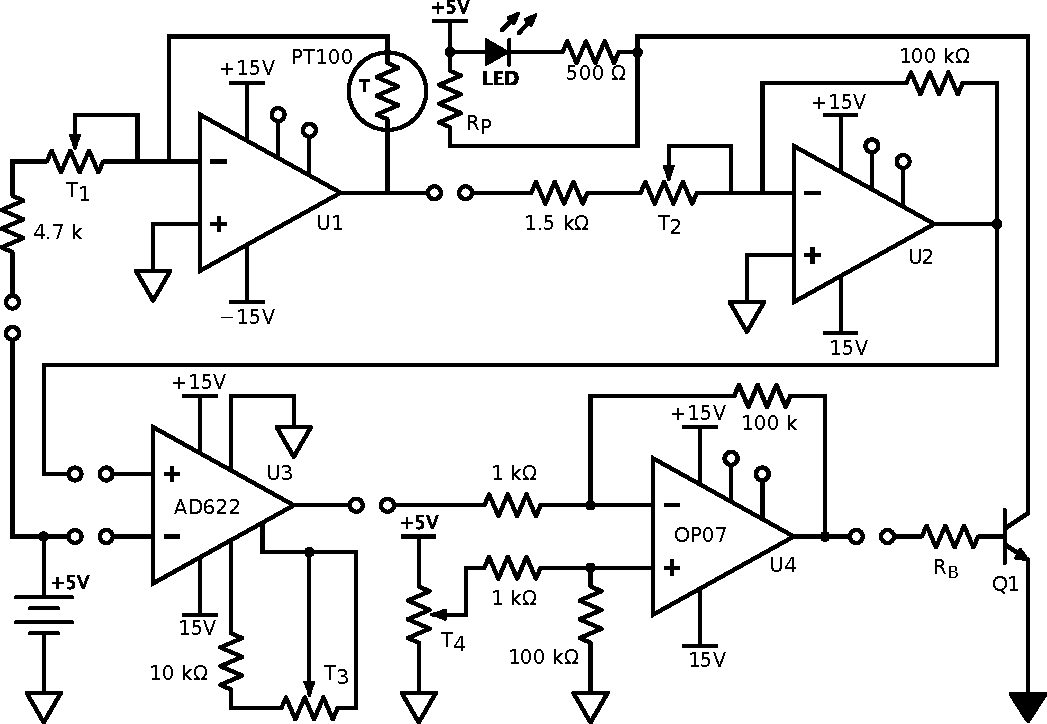
\includegraphics[width=0.75\textwidth]{../E06/latex/c2.pdf}}
 \caption{Schema circuitale del circuito termostatato con termometro elettronico a parallelogramma complesso immerso in criptonite.}
 \label{gr5:a_caso}
\end{figure}
